\subsection*{全体概要：この章で学ぶこと}
\addcontentsline{toc}{subsection}{全体概要：この章で学ぶこと}

この章は、ソフトウェア開発における「設計」を扱う。設計は、要求を実装へ橋渡しする中心的な活動である。要求が「何を満たすべきか」を示すなら、設計は「どのような構造と振る舞いで満たすか」を示す。設計は、プログラムを書く前の一時的な準備だけではなく、保守、変更、品質評価、テスト、認証にも影響する長期的な知識資産である。

\textbf{到達目標} この章を読み終えると、次のことができるようになる。
\begin{itemize}
  \item ソフトウェア設計の意味を、設計という分野、設計活動、設計結果、ライフサイクル上の段階として説明できる。
  \item 設計思考、設計文脈、主要論点、設計原則の役割を説明できる。
  \item 高水準設計と詳細設計の違いを説明できる。
  \item 並行性、イベント処理、データ永続化、分散、例外処理、統合、安全性、変動性など、設計品質の観点を説明できる。
  \item 構造設計記述と振る舞い設計記述の代表的な記法を見分けられる。
  \item 設計パターン、領域固有言語、設計根拠、設計レビュー、設計メトリクスの意味を説明できる。
\end{itemize}

\textbf{学習順序} 初学者は、まず「設計は何を変換する活動か」を押さえる。その後、「よい設計の原則」「設計の段階」「設計で扱う品質」「設計をどう記録するか」「設計方法の違い」「設計をどう評価するか」の順に読むとよい。

\begin{figure}[htbp]
\centering
\IfFileExists{assets/generated_figures/ch03/fig-ch03-01.png}{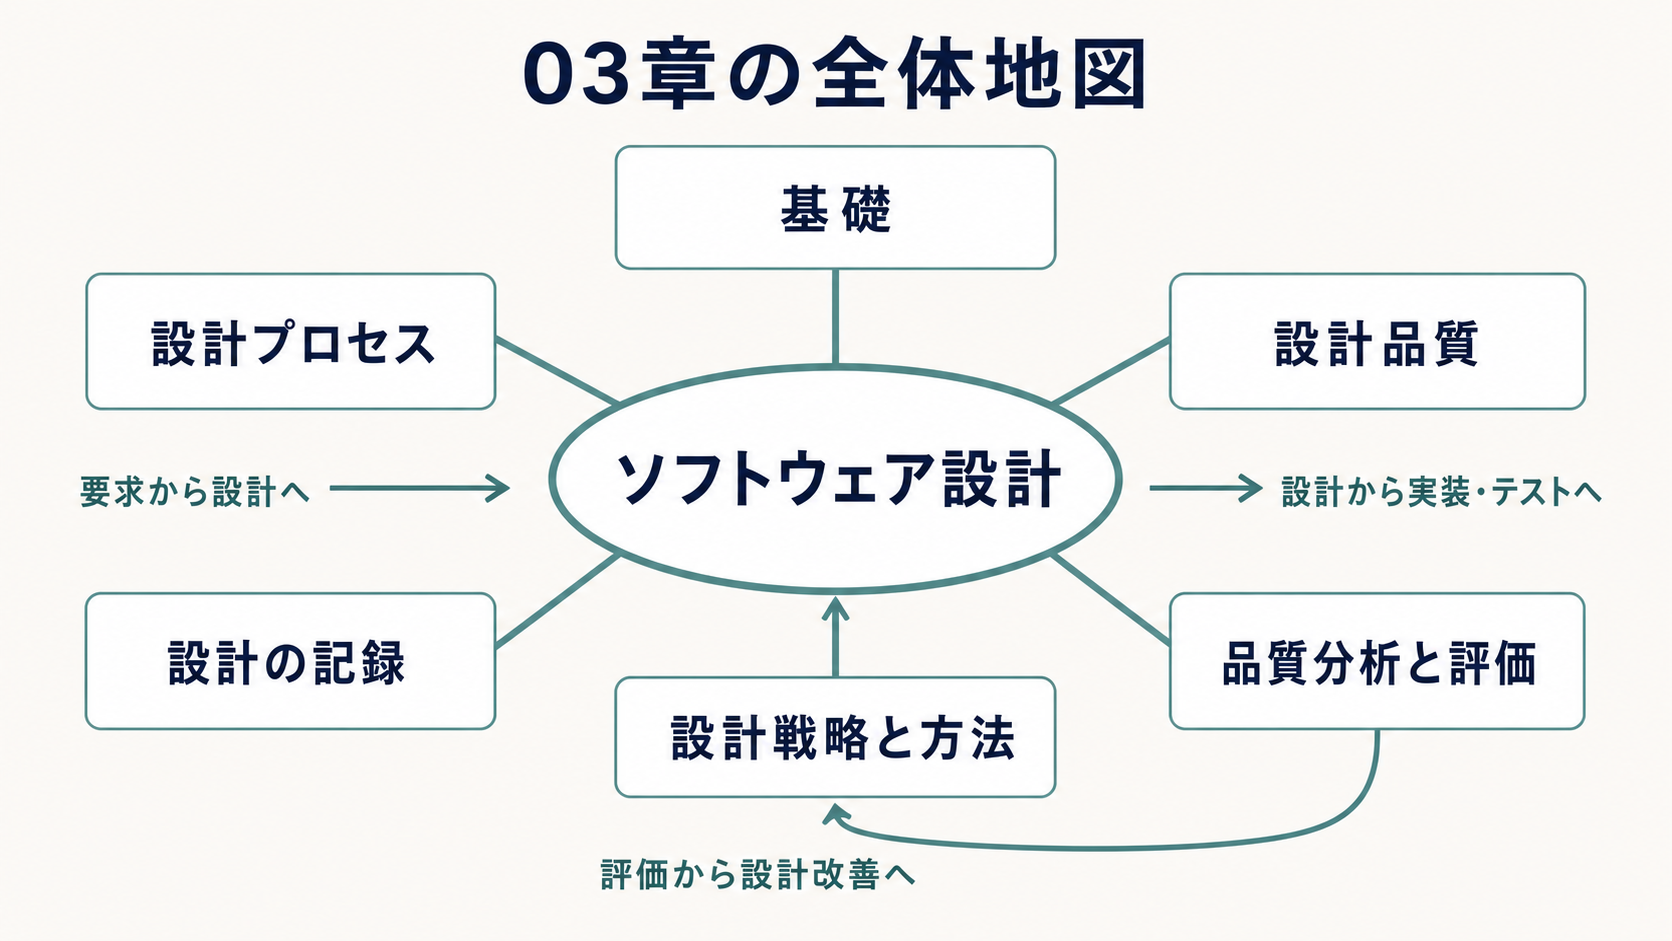
\includegraphics[width=0.96\linewidth]{assets/generated_figures/ch03/fig-ch03-01.png}}{\fbox{\parbox[c][48mm][c]{0.9\linewidth}{\centering 画像生成待ち\\03章の全体地図}}}
\caption{03章の全体地図}
\label{fig:ch03-01}
\end{figure}
